\documentclass[a4paper]{article}
%documentclass[a4paper]{amsart}
\usepackage[a4paper, total={6in, 15in}]{geometry}
\usepackage{siunitx}
\usepackage{physics}
\usepackage{amsmath}
\usepackage{amssymb}
\usepackage{listings}
\usepackage{color}
\usepackage{hyperref}
\usepackage{titling}
\usepackage{epsfig}
\usepackage{ison2022}
\graphicspath{{report/}} 
\definecolor{pythonred}{rgb}{0.6,0,0} % for strings
\definecolor{pythongreen}{rgb}{0.25,0.5,0.35} % comments
\definecolor{pythonpurple}{rgb}{0.5,0,0.35} % keywords
\definecolor{pythondocblue}{rgb}{0.25,0.35,0.75} % pythondoc
\lstset{language=Python, basicstyle=\ttfamily,
keywordstyle=\color{pythonpurple}\bfseries, stringstyle=\color{pythonred},
commentstyle=\color{pythongreen},
morecomment=[s][\color{pythondocblue}]{/**}{*/}, tabsize=4, showspaces=false,
basicstyle=\fontsize{9}{9}\selectfont\ttfamily, showstringspaces=false}


\title{Machine Learning Enabled Venture Capitalism}
\name{Ian Cheung$^1$ \thanks{$^1$ Keble College, Oxford},  Yigit Ihlamu$^2$
\thanks{$^2$ Vela Partners}}
\setlength{\parindent}{0pt}
\setcounter{tocdepth}{2}

\begin{document}
\maketitle

\section*{Abstract}
We used a BERT-based [\ref{BERTpaper}] embedder to embed a dataset of companies ("company
universe") into a 768 dimensional vector ("representation") space. We then
constructed a search engine within this space that queries the universe for best
matches. We found that this performs at accuracy with reasonable speed.
Additionally, we propose a training protocol that allows for model fine-tuning,
which increases both query speed and accuracy for specific tasks.

\tableofcontents

\section{Introduction}
When there is a window of opportunity, entrepreneurs around the world
seek the same opportunities--there is almost never only one
company tackling a problem. For that reason, we built a software suite
("VelaTwins") that allows us to search a database for companies that are alike.
This is particularly necessary for VC firms, who are always looking for (1)
substitute investments and (2) opportunities to diversify within a particular market.

\subsection{Data}
Our dataset contains 655,000 companies and descriptions that are scraped from
websites like \emph{crunchbase}. These companies are split into around 55,000
unique categories, with a median of 10 companies per category. An example
dataset is presented in figure (\ref{datahead}).

\begin{figure}[!h]
    \centerline{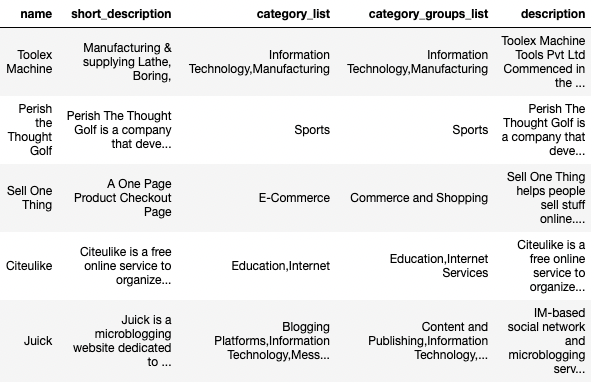
\includegraphics[width=85mm]{datahead.png}}\caption{{\it Dataset}}
    \label{datahead}
\end{figure}


\subsection{Aims and approach}

Given a particular company's description, we want to return a set of $n$ other
companies that are in the same business. Fundamentally, this problem consists of
two different parts: an embedding process (section \ref{embprocess}) to
represent words as computer-readable vectors, and a search process (section
\ref{search}). Fortunately, both of these problems have well-defined solutions.
Since the introduction of word2vec [\ref{word2vecpaper}] in 2013, word-embedding
algorithms have been much improved. Currently, the most effective algorithm is
widely recognised to be Google's BERT, which is a bi-directional transformer.
However, BERT is extremely computationally expensive--for example, running BERT
on our dataset (500 MB) on the author's computer would take up most of his
productive years. Previous attempts at reducing BERT's runtime (e.g. reducing
dataset size via heuristics) came at the cost of accuracy, as well as
introducting human biases. For this project, we used the SBERT
[\ref{sbertpaper}] variation. SBERT is a siamese network built on top of BERT
that reduces runtime by nearly four orders of magnitude while presesrving
BERT-level accuracy. For the search process, we use the industry standard cosine
similarity to search the representation space for the $n$ most similar companies
to the input. 


\section{Model Overview}
Figure \ref{setup} is an overview of the model architecture. The model is built
around the SBERT embedder. For the purposes of demonstration we used the stock
(pretrained) SBERT embedder, although \lstinline{VelaTwins} is also capable of
being re-trained on custom data (detailed in section \ref{training}), which
would greatly increase the overall model accuracy. \lstinline{VelaTwins} is also
built with the settings configured as a shared-state, which allows for the model
parameters to be individually and continuously reconfigured in one step. This
allows for users to fine-tune the model, or indeed, to employ a reinforcement
learning algorithm. This paper is also accompanied by a Jupyter notebook that
demonstrates the capabilities of the model in detail on propietary data.

\begin{figure}[!h]
    \centerline{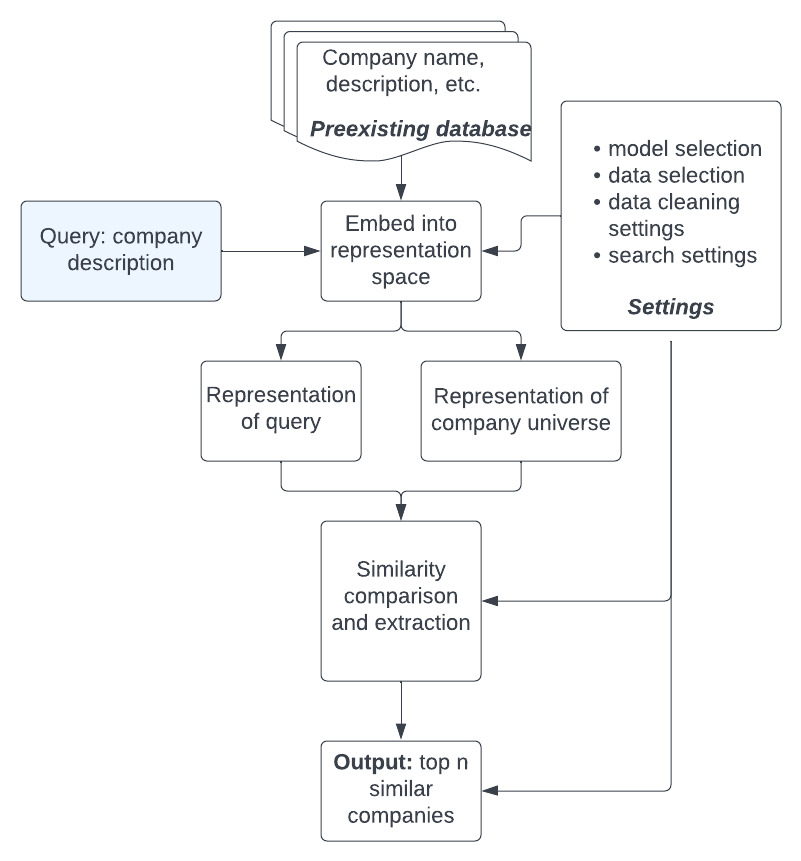
\includegraphics[width=95mm]{uml.jpeg}} \caption{{\it Coarse
    model architecture}}
    \label{setup}
\end{figure}

\subsection{Data Preparation}
To prepare the dataset for our model, we use the module in
\lstinline{Data.config_data}. This takes as an input the raw data (in csv
format) and returns a list of companies along with a description. Descriptions
are cut off after a certain number of words, and "meaningless" words are
also removed (these can be configured in \lstinline{Settings.custom}).
The processed data can then be fed into the embedding process (section \ref{embprocess}).

\subsection{Embedding Process} \label{embprocess} The embedding process in
\lstinline{Model.model} (the vertical flow chart in figure \ref{setup}) should
be run only once during set up. By default, this module uses the pre-trained
SBERT embedder. However, custom embedders can also be used by passing them as
keyword arguments (demonstrated in section \ref{training}). Stock SBERT embeds
the list of companies and descriptions into a representation space of 768
dimensions (each company-description pair is a vector in this space). With the
fine-tuned model in section \ref{training}, this is then passed through a
fully-connected network and condensed down to 256 dimensions. This module
outputs a $d\times n$ matrix where $d$ is the dimension of the representation
space and $n$ is the number of companies in the company universe. This matrix
is then saved for future use.

\subsection{Search Engine}\label{search} The search process is in
\lstinline{Query.query}. It takes a \lstinline{string} input and embeds it into
the same representation space as section \ref{embprocess} using
\lstinline{Model.model}. A cosine similarity matrix is then produced between the
input and every element of the universe, and the top $n$ scores are saved and
the corresponding companies returned. \lstinline{evaluate = True} can be passed
in as a keyword argument, which tells the query model to log
results that are above a certain cosine similarity threshold. Additionally,
\lstinline{evaluate} also returns the SBERT evaluation score, which takes in two
"gold standard" calibration sentences and evaluates the model on whether the
output is close enough to the calibration. The threshold and calibration
sentences are configured in \lstinline{Settings.custom}).

\section{Results}\label{results}
We ran the model on our propietary dataset of 655,000 companies. For
demonstration purposes, we configured the model to return pairs of companies
that are deemed to be correlated. Figure \ref{output} shows one of these pairs.
Note that these two companies are indeed very similar, and provide services that
are almost identical. 

\begin{figure}[!h]
    \centerline{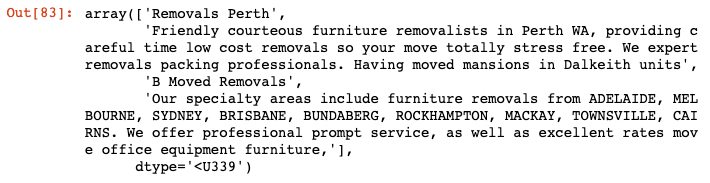
\includegraphics[width=97mm]{output.png}} \caption{{\it Similar sentences}}
    \label{output}
\end{figure}

For a randomly selected set of 50,000 companies in the company universe, we
found 1010 company pairs that are "highly correlated", which we defined to be when the
cosine similarity is over $0.65$. This, combined with the two metrics in section
\ref{search}, can be used for model evaluation. However, due to time
restriction, we were not able to systematically investigate the effects of
different model settings. 

\section{Model Fine Tuning}\label{training} Users of \lstinline{VelaTwins} would
presumably like to use the model on their own datasets. However, datasets are
sometimes dramatically different. As seen in section \ref{results}, stock SBERT
misses out on many results. To address this, we developed a more customisable
embedder built on top of SBERT. The embedder architecture is shown in figure
\ref{train} below. The first two modules within the model, BERT and the pooling
algorithm, are effectively the same as stock SBERT. However, we attach a
fully-connected neural network to the pooling module, which condenses the 768
dimensional vector space into 256 dimensions. This neural network can then be
trained on a specific dataset using \lstinline{Model.train_model} to form
connections that were not immediately obvious to the pre-trained SBERT. The
addition of this dense layer seems to do well in adapting SBERT to specific use
cases, although the user must be careful to avoid overfitting. The use of this
function is strongly recommended if the user has enough training data (see
section \ref{trainingdata}).

\begin{figure}[!h]
    \centerline{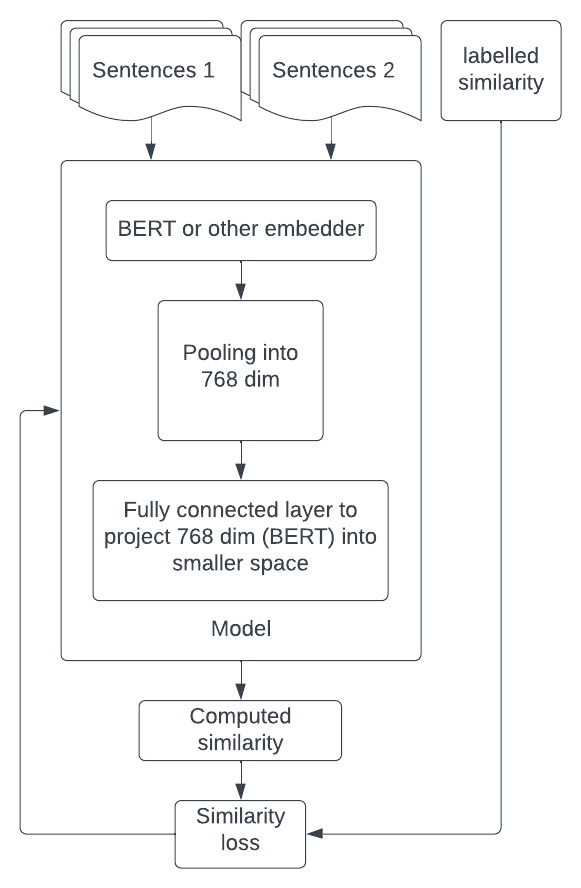
\includegraphics[width=95mm]{training.jpeg}} \caption{{\it Model training}}
    \label{train}
\end{figure}

\subsection{Training data}\label{trainingdata}
As with all simple neural networks, the fully-connected layer needs to be
trained on labelled data. The specific dense layer in \lstinline{VelaTwins}
trains on pairs of companies (in the format of figure \ref{output}), along with
a labelled cosine similarity. The network then compares company pairs and computes a
similarity score, which is passed through to a similarity loss function along
with the labelled similarity. This loss function is minimised during the
training process. \\\\After training, the model can then be saved and passed
through \lstinline{Model.model} to be used as before.
\section{Next steps}
Having built a proof-of-concept, we now look forward to the potential deployment of
the model. However, before that can be done, there are a few issues we need to
address.
\begin{itemize} 
    \item Data Processing: it is not yet obvious what the optimal
    length of the description is, what words should be allowed and what words
    shouldn't, and whether it is wise to pre-filter based on company categories.
    \item Fine-tuning: we currently don't have enough labelled data to properly
    train our fully-connected layer. We are currently in the process of devising
    a method to create a labelled dataset systematically. 
    \item BERT selection: there are different versions of BERT that are trained
    on different datasets (e.g., wikipedia, encyclopedia, etc), and it is not
    yet clear which is optimal.
    \item Automatic data entry: as there are more companies being founded every
    day, we are looking to connect \lstinline{VelaTwins} to automatic data
    collection software, so the company universe can continue expanding.
\end{itemize}

It is clear from this project, though, that the model architecture proposed in
this paper can be used at scale.

\clearpage
\begin{thebibliography}{9}
\bibitem{cmanual}Devlin et al., \emph{BERT: Pre-training of Deep Bidirectional
Transformers}, Google AI,
2019\label{BERTpaper} 
\bibitem{cmanual}Mikolov et al., \emph{Efficient Estimation of Word Representations in Vector Space}, Google,
2013\label{word2vecpaper} 
\bibitem{cmanual}Reimers and Gurevych, \emph{Sentence Embeddings using Siamese BERT-Networks}, Technische Universitat Darmstadt,
2019\label{sbertpaper} 
\end{thebibliography}


\appendix
\renewcommand\thesection{Appendix \Alph{section}}
\end{document}